\chapter{Introduction}

Alzheimer’s disease (AD) is a chronic neurodegenerative disease in which amyloid plaques and neurofibrillary tangles accumulate in the brain. The most common early symptom is the difficulty remembering recent events (short-term memory loss). As the disease advances, patients may lack motivation, have problems with self-care, and show behavioral abnormalities or even withdraw from family and society~\citep{Burns:2009}. AD has a typical pattern of progression, with changes in the brain that correspond to the types and severity of symptoms. Disease progression has commonly been divided into five main categories in the ADNI2 phase of Alzheimer's Disease Neuroimaging initiative(ADNI)~\citep{weiner2013alzheimer}: Cognitively Normal (CN), Significant Memory Concern(SMC), Early Mild Cognitive Impairment (EMCI), Impairment (LMCI) and Alzheimer's Disease (AD), defined clinically based on behavioral and cognitive assessment. (SMC) are self-report significant memory concern from the patient we choose to exclude it from our study. Table.~\ref{fig:participant_stages} shows the participant stages across ADNI 1/2/GO.

There has been a shift with a sense of urgency to find effective intervention in the presymptomatic stage of AD so to reduce the risk of AD, delay or even prevent its onset. To more adequately diagnose different stages of the disease and especially in the early stage and predict future cognitive decline, computer-aided diagnostic classification is increasingly needed using biomarkers based on neuroimaging and other measurements.
There is evidence that the pathogenic cascade of AD is thought to begin at least 1-2 decades prior to cognitive impairment, starting with accumulation of the amyloid-$\beta$1-42(A$\beta$1-42) plaques \citep{langbaum2013ushering}. Research has suggested that these early processes can be assessed using brain imaging and fluid biomarkers. Prior research work on Fluorodeoxyglucose (FDG) positron emission tomography (PET), Pittsburgh compound B (PIB), structural magnetic resonance imaging (sMRI) and functional measures of resting-state networks (rs-fMRI) has supported their validity as potential metabolic biomarkers. Among various neuroimaging techniques, FDG-PET characterizes the cerebral glucose hypometabolism related to AD and those at risk of AD. FDG-PET offers a reliable metabolic biomarker even at pre-symptomatic stages. Despite major advances in FDG-PET used to track symptomatic patients, there is still a lack of sensitive, reliable, and accessible FDG-PET imaging algorithms capable of characterizing abnormal degrees of age-related metabolism decline in preclinical individuals at high risk for AD whom early intervention is most needed. Fig.~\ref{fig:pet_raw} shows the different types of PET scans.

Recently minor cognitive impairment (MCI) in \FDGPET ~has been classified by a brain regional sensitivity mapping method based on summated index (Total Z score) by utilizing the sensitivity-distribution maps~\citep{kakimoto2011new}.In other contemporary works a region of interest (ROI) mask is used to extract features and use incomplete random forest-robust support vector machine to perform classification~\citep{lu2017early}. In general for a classification algorithm based on 3D FDG-PET images the feature dimension is usually much larger than the number of subjects. Data with extremely high dimensionality has presented serious challenges to existing learning methods~\citep{liu2007computational}~\citep{friedman2001elements}. With the presence of a large number of features, a learning model tends to overfit, affecting its performance.

In this context, when we apply three-dimensional statistical maps to do classification the feature dimension is usually much larger than the number of subjects, i.e., the so-called “high dimension, small sample size problem”. When a vast number of variables are measured from a small number of subjects, it is often necessary to reduce their high dimension features to low dimension features. In most cases, the information gets lost by mapping into a lower-dimensional space. However, the discarding information is always compensated by a more accurate space (or feature). There are two general approaches to performing dimensionality reduction: feature selection and feature extraction. Feature selection reduces the feature dimension by selecting a subset of original variables~\citep{jain1997feature}. It aims to choose a small subset of the relevant features from the original ones according to certain relevance evaluation criterion, which usually leads to better learning performance for example higher learning accuracy for classification, lower computational cost, and better model interoperability \citep{tang2014feature}. Feature extraction reduces the dimension based on mathematical projections, which transform the original features into a lower dimensional but more appropriate feature space~\citep{guyon2008feature}. There are some widely used algorithms in machine learning, e.g., principle component analysis (PCA)~\citep{jolliffe2002principal}, linear discriminant analysis (LDA)~\citep{mika1999fisher}, as analytic tools for feature extraction.

Both Feature extraction and feature selection are capable of improving learning performance, lowering computational complexity, building better generalizable models, and decreasing required storage. Feature extraction maps the original feature space to a new feature space with lower dimensions by combining the original feature space. It is difficult to link the features from original feature space to new features. Therefore further analysis of new features is problematic since there is no physical meaning for the transformed features obtained from feature extraction techniques. While feature selection selects a subset of features from the original feature set without any transformation, and maintains the physical meanings of the original features. In this sense, feature selection is superior in terms of better readability and interpretability. This property has its significance in many practical applications such as finding relevant genes to a specific disease and building a sentiment lexicon for sentiment analysis. Typically feature selection and feature extraction are presented separately. Via sparse learning such as $\ell1$ regularization, feature extraction (transformation) methods can be converted into feature selection methods~\citep{masaeli2010transformation}. In order to analyze images more efficiently, a dictionary that allows us to represent them as a superposition of a small number of its elements so that we can reduce each image to a small number of its coefficients~\citep{schnass2008dictionary}. Similarly sparse coding \citep{lin2014stochastic} has been proposed to use a small number of basis vectors (also called dictionary) to represent local features effectively and concisely and help image content recognition. From the input image data, sparse coding learns an over-complete set of basis vectors (dictionary), which have been used to select the most germane features~\citep*{friedman2001elements}. To learn local imaging features, image patches are usually selected to form dictionaries. Dictionary learning and sparse coding \citep{mairal2009online} has shown to be efficient for many tasks such as image deblurring~\citep{yin2008bregman}, image super-resolution~\citep{yin2008bregman} functional connectivity analysis~\cite{lv2015holistic,lv2015modeling}, and image classification (Mairal et al., 2009; Moody et al., 2012). In many computer vision, medical imaging and bioinformatics applications~\citep{mairal2009online,moody2012unsupervised,lv2015modeling} dictionary learning and sparse coding leads to state-of-the-art results.

To address the problem of ``curse of dimensionality'', we propose two sets of approaches for classification of a large set of \FDGPET images, and compare their performance. The first approach consists of a learning based system with sparse coding and dictionary learning for efficient data representation (Feature Learning), maxpooling~\citep{boureau2010theoretical} for feature and again AdaBoost~\citep{rojas2009adaboost} for classification. The second approach is a empirical machine learning based model which includes patch based feature selection then maxpooling~\citep{boureau2010theoretical} for feature agglomeration. We then form data vectors and apply probabilistic principle component analysis for feature extraction using dimension reduction and finally AdaBoost for classification. The two systems serves as a comparison between the approaches for analyzing \FDGPET. Our goal is to discover an appropriate \FDGPET ~diagnosis system design by investigating their performance. We tested our hypothesis on the ADNI2 dataset across $668$ subjects. We then carried out 10 fold cross validation in six different classification experiments comparing the two methods across various imaging measures.

\begin{figure}[h]
	\centering
	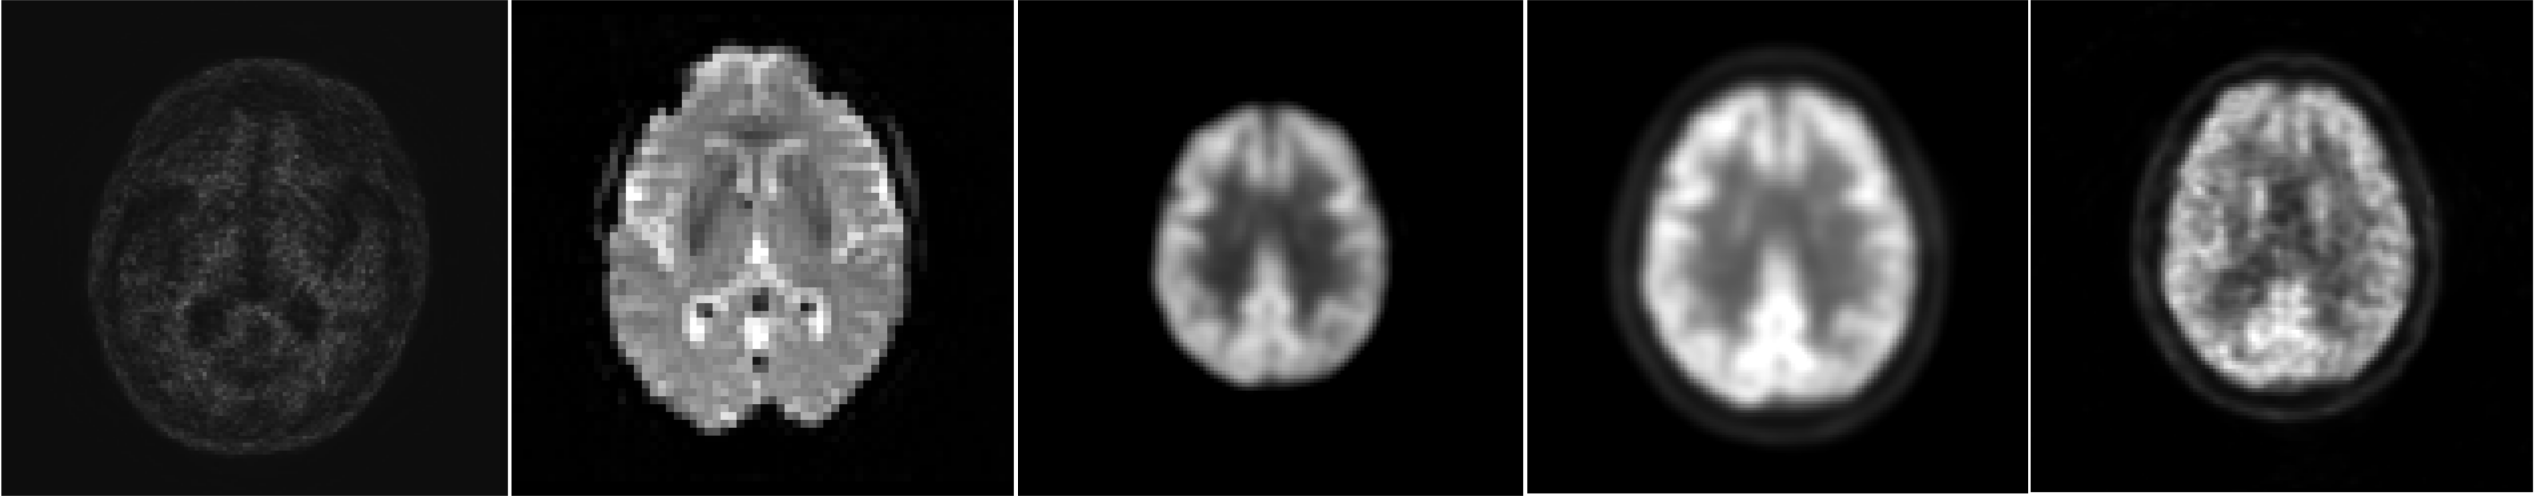
\includegraphics[width=\linewidth]{figures/pet_raw.png}
	\caption{Different types of P.E.T Scans}
	\label{fig:pet_raw}
\end{figure}

{\bf Structure of document} This thesis document is divided logically into the following sections:

\begin{itemize}
	\item Chapter 2 introduces the data used in the preparation of this document and preprocessing of \FDGPET~.
	\item Chapter 3 discusses the background and history of both our proposed methods. It also discuses the role of \FDGPET~as a biomarker. A brief history of the techniques used and motivation. The techniques used are introduced. 
	\item Chapter 4 discusses the system design and architecture in detail and addresses the major components of the system.	
	\item Chapter 5 describes the experimental setup, presents the results and sheds light on the tools analysis. We show the result of classification in both methods. We compare and perform meta-analysis on stochastic coordinate coding (SCC) and dimensionality reduction (feature extraction) and investigate addition of other features. 
	\item Chapter 6 continues our discussion on the results, lessons learned over the course of the project, the limitations and talk about the further improvements.
	\item Chapter 8 concludes the thesis, with ideas about future works.
	
\end{itemize}
	
In this work we shed some light on \FDGPET~as a biomarker and we try to evaluate our statistical map to find a better diagnosis of (AD). In summary we make the following contribution.

\begin{itemize}
	\item We use the second phase of ADNI as our choice of dataset. It is relatively new and has extensive subject information.
	\item Building two empirical series of Machine Learning systems on the above dataset and check the performance of state-of-the art algorithms on \FDGPET.
	\item Introduction of a few demographic features in the classification process which drastically improves performance.     
\end{itemize}    	
	
